\documentclass[12pt,a4paper]{article}
\usepackage{newtxtext,newtxmath}
\usepackage[utf8]{inputenc}
\usepackage[T1]{fontenc}
\usepackage[margin=2.5cm]{geometry}
\usepackage[
backend=biber,
style=apa
]{biblatex}

\addbibresource{referencias.bib}
\usepackage{xcolor}
\usepackage{setspace}
\usepackage{csquotes}
\usepackage{titlesec}

% ---------------------------------------------------------
% DEFINICIÓN DE COLORES
% ---------------------------------------------------------
\definecolor{azulnoche}{RGB}{0,40,90}
\definecolor{celesteclaro}{RGB}{224,240,255}
\definecolor{grisclaro}{RGB}{245,245,245}
\definecolor{darkgreen}{rgb}{0.533, 0.486, 0.184}
\definecolor{golden}{RGB}{197,160,89}
\definecolor{goldford}{RGB}{143,113,54}
\definecolor{rojo}{RGB}{166,25,46}

% ---------------------------------------------------------
% CONFIGURACIÓN DE TÍTULOS
% ---------------------------------------------------------
\titleformat{\section}
{\Huge\bfseries\color{azulnoche}}
{\thesection}
{1em}
{}

\titleformat{\subsection}
{\Large\bfseries\color{azulnoche}}
{\thesubsection}
{1em}
{}

\titleformat{\subsubsection}
{\large\bfseries\color{azulnoche}}
{\thesubsubsection}
{1em}
{}

\usepackage{colortbl}
\usepackage{graphicx}
\usepackage{caption}
\captionsetup{compatibility=false}
\usepackage{booktabs}
\usepackage{tocloft}
\usepackage[spanish,es-tabla]{babel}
\usepackage{hyperref}
\usepackage{float}
\usepackage{tabularx}
\usepackage{array}
\usepackage{listings}

% ---------------------------------------------------------
% CONFIGURACIÓN DE LISTINGS (CÓDIGO JAVA)
% ---------------------------------------------------------
\lstset{
    language=Java,
    basicstyle=\ttfamily\small,
    keywordstyle=\color{azulnoche}\bfseries,
    commentstyle=\color{darkgreen}\itshape,
    stringstyle=\color{rojo},
    numbers=left,
    numberstyle=\tiny\color{gray},
    stepnumber=1,
    numbersep=8pt,
    frame=single,
    rulecolor=\color{azulnoche},
    backgroundcolor=\color{grisclaro},
    breaklines=true,
    showstringspaces=false,
    tabsize=4
}

\hypersetup{
    colorlinks=true,
    linkcolor=azulnoche,
    urlcolor=azulnoche,
    citecolor=azulnoche
}

\setlength{\parindent}{1.5em}
\onehalfspacing
\setlength{\cftbeforesecskip}{6pt}
\renewcommand{\contentsname}{Índice General}

% ---------------------------------------------------------
% ESTILOS DEL ÍNDICE CON COLORES RESPETADOS
% ---------------------------------------------------------
\renewcommand{\cftsecfont}{\color{azulnoche}\bfseries}
\renewcommand{\cftsubsecfont}{\color{azulnoche}}
\renewcommand{\cftsubsubsecfont}{\color{azulnoche}\itshape}

\renewcommand{\cftsecpagefont}{\color{azulnoche}\bfseries}
\renewcommand{\cftsubsecpagefont}{\color{azulnoche}}
\renewcommand{\cftsubsubsecpagefont}{\color{azulnoche}}

\renewcommand{\cftsecpresnum}{\color{azulnoche}}
\renewcommand{\cftsubsecpresnum}{\color{azulnoche}}
\renewcommand{\cftsubsubsecpresnum}{\color{azulnoche}}

\renewcommand{\cftsecaftersnum}{\color{azulnoche}}
\renewcommand{\cftsubsecaftersnum}{\color{azulnoche}}
\renewcommand{\cftsubsubsecaftersnum}{\color{azulnoche}}

\begin{document}

% =========================================================
% CARÁTULA
% =========================================================

\begin{titlepage}
\centering
{\color{golden}\bfseries\large UNIVERSIDAD NACIONAL MAYOR DE SAN MARCOS}\\
\vspace{0.2cm}
{\color{golden}\large\textbf{Universidad del Perú, Decana de América}}\\
\vspace{0.6cm}

\includegraphics[width=0.5\textwidth]{LOGOUNMSM.png}\\
\vspace{0.5cm}
{\color{goldford}\scshape\Large Facultad de Ingeniería de Sistemas e Informática\\}
{\color{goldford}\scshape\large Escuela Profesional de Ingeniería de Sistemas\\}
\vspace{0.6cm}
\color{rojo}\hrule height 0.3mm\vspace{0.5cm}
{\color{rojo}\Large\bfseries Semana 1 - POO\vspace{0.56cm}}\\
\color{rojo}\hrule height 0.3mm\vspace{0.6cm}
{\color{rojo}\Large\textbf{Curso:}}\\
\vspace{0.2cm}
{\color{goldford}\Large Programación de Computadoras II}\\
\vspace{0.7cm}
{\color{rojo}\Large\textbf{Docente:}}\\
\vspace{0.2cm}
{\color{goldford}\Large Javier Elmer Cabrera Díaz}\\
\vspace{0.7cm}
{\color{rojo}\Large\textbf{Autor:}}\\
\vspace{0.2cm}
{\color{goldford}\Large Mamani Huahualuque, Airton Abedal}\\
\vspace{1.5cm}
{\color{goldford}\Large\textbf{Lima, 31 de Agosto del 2026}}\\
\end{titlepage}

% =========================================================
% ÍNDICE
% =========================================================

\newpage
\pagenumbering{arabic}
\setcounter{page}{1}

\tableofcontents

\newpage

% =========================================================
% 1. INTRODUCCIÓN
% =========================================================

\section{Introducción}

La presente tarea corresponde a la primera semana del curso de
Programación 2 y tiene como eje la transición desde la programación
estructurada hacia la Programación Orientada a Objetos (POO).

De acuerdo con el material de clase, Programación 1 se relaciona con
la programación estructurada, incluyendo secuencia, alternativa,
estructuras repetitivas, modularidad y archivos. Por otro lado,
Programación 2 introduce la Programación Orientada a Objetos, cuyo
enfoque permite representar elementos del mundo real mediante
objetos relacionados.

Los principales conceptos de la POO que se presentan en esta etapa
son la abstracción, el encapsulamiento, la herencia y el polimorfismo.

A partir de esta introducción, el presente trabajo desarrolla cinco
actividades planteadas por el docente: un sumario de cuatro
herramientas CASE relacionadas con la ingeniería de software; una
comparación entre \texttt{struct} y \texttt{class}; la ampliación de
la prueba realizada en el método \texttt{main()} del ejemplo de la
clase; una revisión de los tipos de datos de Java; y la explicación
del resultado negativo obtenido al sumar dos valores enteros de gran
magnitud.

El objetivo es comprender no solamente la sintaxis utilizada en
Java, sino también los conceptos que justifican la organización de
un programa mediante clases y objetos.

En particular, el caso de la clase \texttt{TV} permite relacionar
atributos, métodos, creación de instancias, validación de datos y
encapsulamiento con una situación concreta.

% =========================================================
% 2. DESARROLLO
% =========================================================

\section{Desarrollo}

% ---------------------------------------------------------
% 2.1 CASE
% ---------------------------------------------------------

\subsection{Sumario de cuatro herramientas CASE}

CASE (\textit{Computer-Aided Software Engineering}) es el término
utilizado para referirse a herramientas informáticas que apoyan
distintas actividades de la ingeniería de software.

Dependiendo de la herramienta, pueden facilitar el análisis,
modelado, diseño, documentación, generación de código, gestión del
proyecto u otras actividades relacionadas con el ciclo de desarrollo
de software.

\subsubsection{StarUML}

StarUML es una herramienta orientada al modelado de sistemas
mediante UML. Permite elaborar diferentes tipos de diagramas, como
diagramas de clases, casos de uso, secuencia, actividad y
componentes.

Es especialmente útil para representar visualmente la estructura y
el comportamiento de un sistema antes de implementar el código.

\textbf{Aplicación en POO:}

En el contexto de Programación Orientada a Objetos, puede utilizarse
para diseñar clases, identificar atributos y métodos y representar
las relaciones existentes entre diferentes clases.

\subsubsection{Visual Paradigm}

Visual Paradigm es una herramienta de ingeniería de software que
ofrece capacidades de modelado UML y apoyo a diferentes actividades
del desarrollo.

Permite trabajar con distintos tipos de diagramas y documentar
modelos del sistema.

\textbf{Aplicación en POO:}

Puede emplearse para pasar de una representación conceptual del
sistema a una especificación más detallada de las clases y sus
relaciones.

\subsubsection{Enterprise Architect}

Enterprise Architect es una herramienta de modelado y diseño de
sistemas utilizada para trabajar con UML y otros modelos
relacionados con el desarrollo de software.

Está orientada a proyectos donde se necesita documentar y administrar
modelos de manera amplia.

\textbf{Aplicación en POO:}

En un proyecto de POO permite representar clases, interfaces,
herencia, asociaciones y otras relaciones que posteriormente pueden
ser implementadas en Java u otro lenguaje.

\subsubsection{ArgoUML}

ArgoUML es una herramienta de modelado UML de código abierto,
utilizada para crear modelos y diagramas de software.

Su enfoque está relacionado principalmente con el modelado y la
representación de estructuras de software.

\textbf{Aplicación en POO:}

Puede servir como recurso académico para practicar la identificación
de clases, atributos, operaciones y relaciones antes de escribir la
implementación.

% ---------------------------------------------------------
% TABLA CASE
% ---------------------------------------------------------

\subsubsection{Comparación general}

\begin{table}[H]
\centering
\caption{Comparación de herramientas CASE}
\renewcommand{\arraystretch}{1.3}

\begin{tabular}{p{3cm} p{3.5cm} p{4.5cm} p{3cm}}
\toprule
\textbf{Herramienta} &
\textbf{Enfoque principal} &
\textbf{Utilidad en POO} &
\textbf{Tipo} \\
\midrule

StarUML &
Modelado UML &
Diseño de clases y relaciones &
Herramienta CASE/modelado \\

Visual Paradigm &
Modelado y desarrollo &
Modelos UML y documentación &
Herramienta CASE \\

Enterprise Architect &
Modelado y arquitectura &
Clases, interfaces y relaciones &
Herramienta CASE \\

ArgoUML &
Modelado UML &
Práctica de estructuras y diagramas &
Herramienta CASE de código abierto \\

\bottomrule
\end{tabular}

\end{table}

% ---------------------------------------------------------
% 2.2 STRUCT VS CLASS
% ---------------------------------------------------------

\subsection{Struct vs. Class}

La comparación entre \texttt{struct} y \texttt{class} depende del
lenguaje de programación. En el contexto de la tarea, la comparación
es especialmente útil para diferenciar una estructura de datos de
una clase utilizada en Programación Orientada a Objetos.

En lenguajes como C++, \texttt{struct} y \texttt{class} pueden
utilizarse para definir tipos que agrupan datos y funciones.

Una diferencia fundamental es el nivel de acceso predeterminado:
en una \texttt{struct} de C++, los miembros son públicos por defecto,
mientras que en una \texttt{class} son privados por defecto.

También es posible utilizar herencia con ambos mecanismos.

En Java no existe la palabra reservada \texttt{struct}. Para crear
tipos definidos por el programador se utiliza principalmente
\texttt{class}, además de interfaces, enumeraciones y otros
mecanismos.

Por ello, cuando el curso trabaja Programación Orientada a Objetos
en Java, la clase es el mecanismo central para representar objetos.

\begin{table}[H]
\centering
\caption{Comparación entre struct y class}
\renewcommand{\arraystretch}{1.3}

\begin{tabular}{p{3.5cm} p{4.5cm} p{5cm}}
\toprule
\textbf{Aspecto} &
\textbf{struct (C++)} &
\textbf{class (Java/C++)} \\
\midrule

Existencia en Java &
No existe como palabra reservada &
Sí, es el mecanismo principal para definir clases \\

Acceso predeterminado en C++ &
\texttt{public} &
\texttt{private} \\

Uso típico &
Agrupar datos y funciones &
Modelar entidades/objetos y encapsular comportamiento \\

POO &
Puede participar en POO en C++ &
Es fundamental para POO en Java \\

Instancias &
Se pueden crear objetos en C++ &
Se crean objetos mediante \texttt{new} en Java \\

\bottomrule
\end{tabular}

\end{table}

En conclusión, para el curso de Programación 2 en Java, la
comparación sirve principalmente para comprender que Java trabaja
con clases como base de la abstracción y la creación de objetos,
mientras que \texttt{struct} es un concepto propio de otros
lenguajes como C/C++.

% ---------------------------------------------------------
% 2.3 MAIN
% ---------------------------------------------------------

\subsection{Ampliación de la prueba en el método main()}

El ejemplo de la clase utiliza una clase \texttt{TV} con tres
atributos: \texttt{canal}, \texttt{volumen} y \texttt{on}.

Además, define operaciones para encender y apagar el televisor,
subir y bajar el canal y establecer un canal válido.

El programa crea dos instancias, \texttt{tv1} y \texttt{tv2}, lo que
permite demostrar que dos objetos pertenecen a la misma clase, pero
mantienen su propio estado.

Una ampliación útil del método \texttt{main()} consiste en probar
más operaciones y comprobar los límites establecidos por la clase.

\begin{figure}[H]
    \centering
    % Enlace a la imagen guardada en tu proyecto
    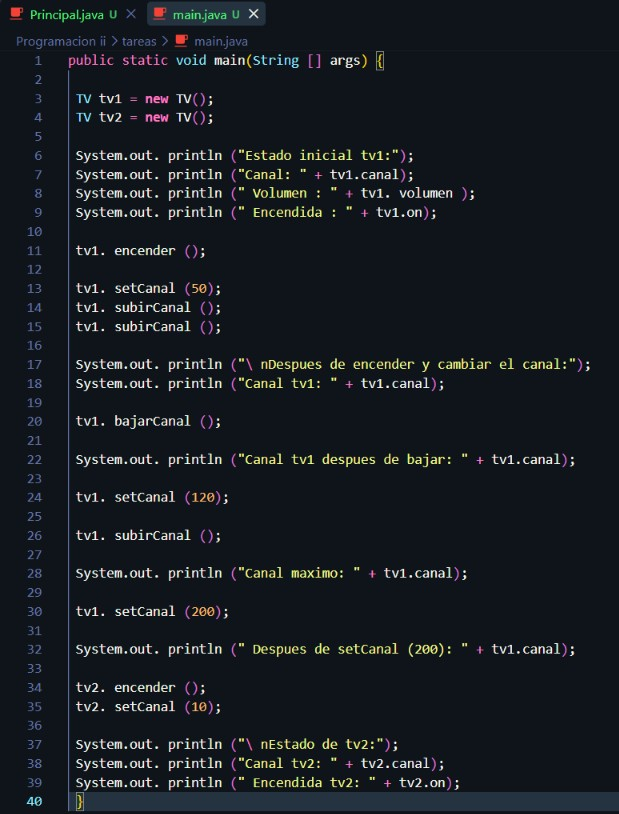
\includegraphics[width=0.85\textwidth]{codigo1.jpg} 
    
    \caption*{
        \raggedright
        {\bfseries Figura 1}\\
        {\itshape Ampliación del método main() para validar el comportamiento y límites de la clase TV}
    }
    
    \vspace{0.2cm}
    
    \begin{raggedright}
    \small {\itshape Nota.} Captura de pantalla de la implementación del método \texttt{main()} en el entorno de desarrollo, donde se evalúa la independencia de estados entre objetos y los límites de los métodos de control. 
    Elaboración propia.
    \end{raggedright}
\end{figure}

Esta prueba permite observar una idea central de POO: cada objeto
posee su propio estado.

Aunque \texttt{tv1} y \texttt{tv2} fueron creados a partir de la
misma clase \texttt{TV}, cambiar el canal de \texttt{tv1} no cambia
el canal de \texttt{tv2}.

% ---------------------------------------------------------
% 2.4 TIPOS DE DATOS
% ---------------------------------------------------------

\subsection{Tipos de datos en Java}

Java posee tipos de datos primitivos y tipos de referencia.

Los tipos primitivos representan valores básicos, mientras que los
tipos de referencia permiten trabajar con objetos, arreglos,
cadenas y otros tipos definidos por el programador.

\begin{table}[H]
\centering
\caption{Principales tipos de datos en Java}
\renewcommand{\arraystretch}{1.3}

\begin{tabular}{p{2cm} p{2.5cm} p{3.5cm} p{5cm}}
\toprule
\textbf{Tipo} &
\textbf{Categoría} &
\textbf{Ejemplo} &
\textbf{Descripción} \\
\midrule

\texttt{byte} &
Entero &
\texttt{byte x = 100;} &
Entero pequeño con signo \\

\texttt{short} &
Entero &
\texttt{short x = 1000;} &
Entero con rango mayor que byte \\

\texttt{int} &
Entero &
\texttt{int x = 200;} &
Entero de 32 bits \\

\texttt{long} &
Entero &
\texttt{long x = 200L;} &
Entero de 64 bits \\

\texttt{float} &
Decimal &
\texttt{float x = 2.5f;} &
Decimal de precisión simple \\

\texttt{double} &
Decimal &
\texttt{double x = 2.5;} &
Decimal de doble precisión \\

\texttt{char} &
Carácter &
\texttt{char c = 'A';} &
Representa un carácter Unicode \\

\texttt{boolean} &
Lógico &
\texttt{boolean ok = true;} &
Representa \texttt{true} o \texttt{false} \\

\texttt{String} &
Referencia &
\texttt{String s = "Hola";} &
Cadena de caracteres; es una clase \\

\bottomrule
\end{tabular}

\end{table}

Para el ejemplo de la clase, el tipo \texttt{int} es especialmente
importante porque su capacidad es finita.

Un \texttt{int} de Java ocupa 32 bits y utiliza representación con
signo, por lo que su rango va desde:

\[
-2\,147\,483\,648
\]

hasta:

\[
2\,147\,483\,647
\]

% ---------------------------------------------------------
% 2.5 OVERFLOW
% ---------------------------------------------------------

\subsection{¿Por qué se obtiene a+b = -294967296?}

El código planteado en la clase es:

\begin{figure}[H]
    \centering
    % Enlace a la imagen guardada en tu proyecto
    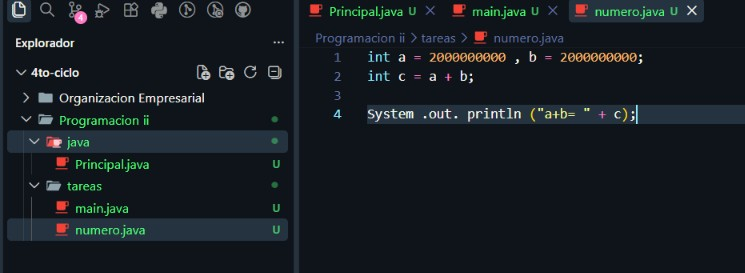
\includegraphics[width=0.93\textwidth]{codigo2.jpg} 
    
    \caption*{
        \raggedright
        {\bfseries Figura 2}\\
        {\itshape Código fuente para la demostración de desbordamiento aritmético en Java}
    }
    
    \vspace{0.2cm}
    
    \begin{raggedright}
    \small {\itshape Nota.} Captura del archivo \texttt{numero.java} en el entorno de desarrollo, donde se define la suma de dos variables de tipo \texttt{int} que superan el límite superior de representación de 32 bits. Elaboración propia.
    \end{raggedright}
\end{figure}

Matemáticamente, la suma de los dos valores es:

\[
2\,000\,000\,000
+
2\,000\,000\,000
=
4\,000\,000\,000
\]

Sin embargo, ese resultado no puede representarse como un valor
positivo dentro del rango de un \texttt{int}, cuyo máximo es:

\[
2\,147\,483\,647
\]

Por esta razón ocurre un \textbf{overflow} o desbordamiento
aritmético.

El resultado matemático:

\[
4\,000\,000\,000
\]

se encuentra fuera del rango representable por un entero
\texttt{int} de 32 bits.

Debido a la representación binaria con complemento a dos utilizada
para los enteros con signo, los bits resultantes corresponden al
valor:

\[
-294\,967\,296
\]

Por eso Java muestra:

\begin{verbatim}
a+b= -294967296
\end{verbatim}

\subsubsection{Representación conceptual}

El problema puede resumirse de la siguiente manera:

\begin{verbatim}
2,000,000,000 + 2,000,000,000 = 4,000,000,000
\end{verbatim}

Mientras que el rango de \texttt{int} es:

\[
-2\,147\,483\,648
\leq
\texttt{int}
\leq
2\,147\,483\,647
\]

Como:

\[
4\,000\,000\,000
>
2\,147\,483\,647
\]

el resultado no puede ser almacenado correctamente como un
\texttt{int} positivo.

\subsubsection{Solución utilizando long}

Una forma de evitar el problema es utilizar el tipo \texttt{long},
que posee un rango mucho mayor:

\begin{figure}[H]
    \centering
    % Enlace a la imagen guardada en tu proyecto
    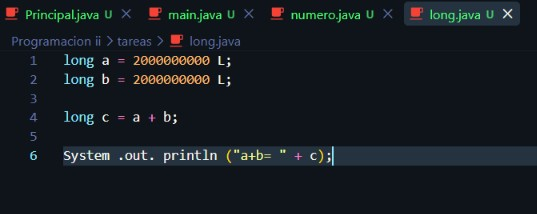
\includegraphics[width=0.85\textwidth]{codigo3.jpg} 
    
    \caption*{
        \raggedright
        {\bfseries Figura 3}\\
        {\itshape Solución al desbordamiento mediante el uso del tipo de dato long}
    }
    
    \vspace{0.2cm}
    
    \begin{raggedright}
    \small {\itshape Nota.} Captura del archivo \texttt{long.java} en el IDE, donde se declaran variables de tipo \texttt{long} con el sufijo \texttt{L} para prevenir el desbordamiento numérico y almacenar correctamente la suma. Elaboración propia.
    \end{raggedright}
\end{figure}

La salida esperada es:

\begin{verbatim}
a+b= 4000000000
\end{verbatim}

Es importante agregar la letra \texttt{L} a los literales cuando se
desea expresar explícitamente que el valor es de tipo \texttt{long}.

También debe almacenarse el resultado en una variable \texttt{long}.

% ---------------------------------------------------------
% 2.6 TV
% ---------------------------------------------------------

\subsection{Relación con el caso de la clase TV}

El caso \texttt{TV} resume varios conceptos iniciales de POO.

La clase define atributos como \texttt{canal}, \texttt{volumen} y
\texttt{on}, mientras que sus métodos representan acciones.

La creación de \texttt{tv1} y \texttt{tv2} mediante
\texttt{new TV()} demuestra la creación de instancias.

Además, los métodos \texttt{subirCanal()} y
\texttt{bajarCanal()} contienen condiciones que impiden salir de
los límites establecidos para el canal.

El método \texttt{setCanal()} valida que el canal se encuentre entre
1 y 120.

Este mecanismo constituye una primera aproximación al
\textbf{encapsulamiento}, concepto que será profundizado mediante
atributos privados, getters y setters.

\begin{figure}[H]
    \centering
    % Enlace a la imagen guardada en tu proyecto
    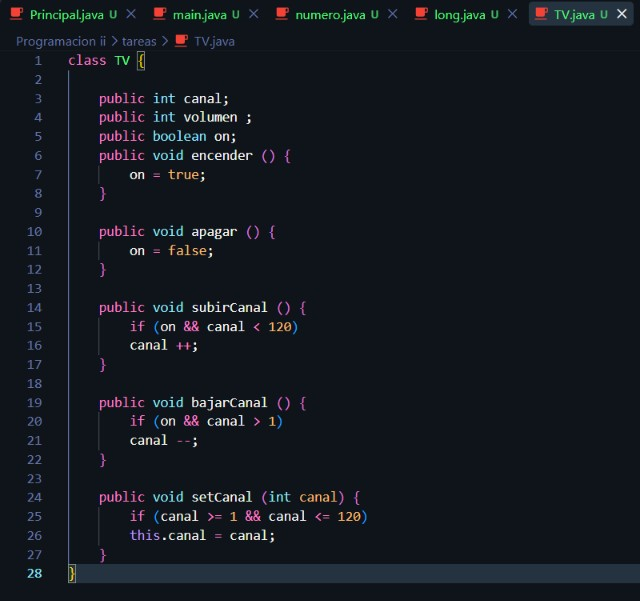
\includegraphics[width=0.85\textwidth]{codigo4.jpg} 
    
    \caption*{
        \raggedright
        {\bfseries Figura 4}\\
        {\itshape Implementación de la clase TV con atributos, métodos de control y validación de límites}
    }
    
    \vspace{0.2cm}
    
    \begin{raggedright}
    \small {\itshape Nota.} Captura del archivo \texttt{TV.java} en el entorno de desarrollo, donde se definen los atributos de estado, métodos de encendido/apagado y la lógica condicional para el cambio de canales. Elaboración propia.
    \end{raggedright}
\end{figure}

% =========================================================
% 3. CONCLUSIÓN
% =========================================================
\newpage
\section{Conclusión}

El desarrollo de esta tarea permitió reforzar los conceptos iniciales
presentados en la primera clase de Programación 2.

La transición de la programación estructurada hacia la Programación
Orientada a Objetos implica una nueva forma de organizar el software,
donde las clases permiten definir tipos y los objetos representan
instancias concretas con atributos y métodos.

El estudio de las herramientas CASE permitió identificar su utilidad
como apoyo a la ingeniería de software, especialmente para modelar,
documentar y representar sistemas antes o durante su implementación.

La comparación entre \texttt{struct} y \texttt{class} mostró que el
concepto depende del lenguaje y que, en Java, la clase constituye el
mecanismo fundamental para construir tipos orientados a objetos.

Asimismo, la ampliación del método \texttt{main()} permitió comprobar
experimentalmente el comportamiento de los objetos \texttt{TV} y
observar que cada instancia mantiene su propio estado.

Finalmente, el análisis de los tipos de datos de Java permitió
comprender que los tipos numéricos poseen límites.

El caso de la suma de dos valores \texttt{int} demuestra el fenómeno
de overflow y explica por qué una operación matemáticamente positiva
puede producir un resultado negativo cuando el valor supera la
capacidad del tipo de dato.

En conjunto, estos conceptos constituyen una base necesaria para los
siguientes temas del curso, entre ellos la sobrecarga de constructores,
\texttt{toString()}, encapsulamiento mediante getters y setters,
relaciones entre clases, clases abstractas e interfaces.

% =========================================================
% 4. REFERENCIAS
% =========================================================

\section{Referencias}

\begin{itemize}

    \item Material de clase: \textit{PROGRA 2 - S1 - 27 agosto.txt},
    proporcionado para la primera semana del curso.

    \item Archivo de demostración:
    \textit{PROGRA2\_DEMOTV.java}, proporcionado para la primera
    semana del curso.

    \item Documentación y conocimientos generales sobre Java, UML y
    herramientas CASE utilizados como complemento explicativo.

\end{itemize}

\end{document}